\documentclass[11pt]{article}
\usepackage[hmargin=1in,vmargin=1in]{geometry}
\usepackage{xcolor}
\usepackage{amsmath}
\usepackage{graphicx} % Required for inserting images
\usepackage{amsmath,amssymb,amsfonts,url,sectsty,framed,tcolorbox,framed}
\usepackage{nicematrix}
\usepackage{amssymb}
\usepackage{algorithm2e}
\setcounter{MaxMatrixCols}{16}
\usepackage{tikz}
\usepackage{hyperref}
\usetikzlibrary{decorations.pathreplacing}
\newcommand{\pf}{{\bf Proof: }}
\newtheorem{theorem}{Theorem}
\newtheorem{lemma}{Lemma}
\newtheorem{proposition}{Proposition}
\newtheorem{definition}{Definition}
\newtheorem{remark}{Remark}
\newcommand{\zbar}{\raisebox{0.2ex}{--}\kern-0.6em Z}
\newcommand{\qed}{\hfill \rule{2mm}{2mm}}
\usepackage{titlesec}

\setcounter{secnumdepth}{4}
\titleclass{\subsubsubsection}{straight}[\subsection]
\newcounter{subsubsubsection}[subsubsection]
\renewcommand{\thesubsubsubsection}{\thesubsubsection.\arabic{subsubsubsection}}
\titleformat{\subsubsubsection}{\normalfont\normalsize\bfseries}{\thesubsubsubsection}{1em}{}
\titlespacing*{\subsubsubsection}{0pt}{3.25ex plus 1ex minus .2ex}{1.5ex plus .2ex}

\setcounter{tocdepth}{4}

\begin{document}



%%%%%%%%%%%%%%%%%%%%%%%%%%%%%%%%%%%%%%%%%%%%%%%%%%%%%%%%%%%%%%%%%%%%%
\noindent
\rule{\textwidth}{1pt}
\begin{center}
{\bf [CS304] Introduction to Cryptography and Network Security}
\end{center}
Course Instructor: Dr. Dibyendu Roy \hfill Winter 2022-2023\\
Scribed by: Chitranshi Srivastava (202051055) \hfill Lecture 22 (Week 12)
\\
\rule{\textwidth}{1pt}
%%%%%%%%%%%%%%%%%%%%%%%%%%%%%%%%%%%%%%%%%%%%%%%%%%%%%%%%%%%
%write here

\section{Elliptic Curve Digital Signature Algorithm(ECDSA)}
Let us first recall that:\\
\textbf{RSA-Signature}:\\
\begin{itemize}
    \item RSA Encryption/Decryption:\\
    Encryption : c = $x^e$ mod n\\
    Decryption : x = $c^d$ mod n\\

    \item Signature :\\
    Signature : s = $x^d$ mod n\\
    Verification : x = $s^e$ mod n\\
\end{itemize}
In ECDSA, we have (E, P) as public keys.\\
\begin{center}
    Secret Key : a\\
    Public Key : aP\\
\end{center}
Here, we need 
\begin{itemize}
    \item elliptic curve EC
    \item a base point-G on the curve. G is such that there exists a large prime number n, such that
\end{itemize}
\begin{center}
    $n\cdot G = 0$\\
    $\implies$ $(n-1)G\ \boxed{+} G\ =\ nG$\\
\end{center}
\begin{center}
    Secret Key : $d_A$\\
    Public Key $Q_A$ : $d_A \cdot G$
\end{center}
Now let us see a scenarios between Alice and Bob:
\begin{center}
    

\tikzset{every picture/.style={line width=0.75pt}} %set default line width to 0.75pt        

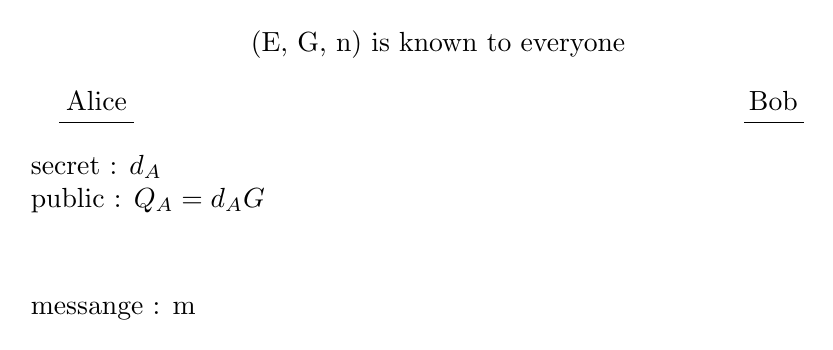
\begin{tikzpicture}[x=0.75pt,y=0.75pt,yscale=-1,xscale=1]
%uncomment if require: \path (0,300); %set diagram left start at 0, and has height of 300

%Straight Lines [id:da1435011466169438] 
\draw    (137,64.4) -- (173,64.4) ;
%Straight Lines [id:da7210376025319416] 
\draw    (467,64.4) -- (496,64.4) ;

% Text Node
\draw (139,48) node [anchor=north west][inner sep=0.75pt]   [align=left] {Alice};
% Text Node
\draw (468,48) node [anchor=north west][inner sep=0.75pt]   [align=left] {Bob};
% Text Node
\draw (122,79) node [anchor=north west][inner sep=0.75pt]   [align=left] {secret : $d_A$\\public : $Q_A = d_AG$};
% Text Node
\draw (228,19) node [anchor=north west][inner sep=0.75pt]   [align=left] {(E, G, n) is known to everyone};
% Text Node
\draw (122,150) node [anchor=north west][inner sep=0.75pt]   [align=left] {messange : m};


\end{tikzpicture}
\end{center}
\subsection{Process of Signature}
Let us now see the \textbf{Process of Signature}:
\begin{enumerate}
    \item e = Hash(m)
    \item \zbar $\rightarrow\ L_n$ leftmost bits of e when $L_n$ is the bit length of n
    \item K $\rightarrow$ randomly from [1, n-1]
    \item $(x_1, y_1)$ = K$\cdot$G\\
    \item r = $x_1$ mod n\\
    if r = 0 then go to step 3\\
    \item $s\ =\ K^{-1}$ [ \zbar + $r \cdot d_A $  ] mod n\\
    if s = 0, then go to step 3
    \item Signature (r, s) on message m
\end{enumerate}
\subsection{Verification of ECDSA}
Let us now see \textbf{Verification of ECDSA} performed by Bob:
\begin{enumerate}
    \item $Q_A$ is not equal to 0
    \item $Q_A$ lies on the curve EC or not
    \item $n\times Q_A$ = $n \cdot (d_A \cdot G)$ = $d_A \cdot (n \cdot G)$ = 0
    \item verify r, s $\in$ [1, n-1]
    \item e = Hash(m)
    \item \zbar $\ \rightarrow\ L_n$ leftmost bits of e
    \item $u_1 \ =\ $ \zbar$\cdot s^{-1}$ mod n\\
    $u_2\ =\ r \cdot s^{-1}$ mod n
    \item $(x_2, y_2)\ =\ u_1G\ +\ u_2Q_A$\\
    if $(x_2, y_2)$ = 0, then signature is invalid. Here addition is addition on the curve.
    \item If r $\equiv\ x_2$ mod n, then signature is valid, otherwise invalid.
\end{enumerate}
Let us see the proof now:\\
\begin{center}
    c = $u_1G\ +\ u_2Q_A$\\
    c = $u_1G\ +\ u_2d_AG$\\
    c = $(u_1\ +\ u_2d_A)$G\\
    c = (\zbar$\cdot s^{-1}\ +\ rs^{-1}d_A)$G\\
    c = (\zbar $\ +\ rd_A)s^{-1}$G\\
    Substituting $s^{-1}$\\
    c = (\zbar $\ +\ r\cdot d_A){(K^{-1}(\zbar\ +\ r\cdot d_A))}^{-1}$G\\
    c = (\zbar $\ +\ r\cdot d_A){(\zbar\ +\ r \cdot d_A)}^{-1}$KG\\
    c = K$\cdot$G
\end{center}
Hence, proved.

It is not the general form of the Elliptic Curve. In fact, we will not be using this curve for practical purposes.

\section{ElGamal Public Key Cryptosystem}
It is a public key encryption algorithm like RSA. Unlike RSA, the security of ElGamal Encryption is based on the Discrete Log Problem. The steps below presents a detailed explanation of the encryption and decryption process.
\begin{enumerate}
    \item Select a prime p.
    \item Consider the group $(Z_p^*, *_p)$.
    \begin{center}
        $Z_p^* = \{1,2,3,\hdots,(p-1)\}$\\
        \vspace{1mm}
        $x *_p y = x * y (mod \ p)$\\
        \vspace{1mm}
    \end{center}
    If $x \in Z_p^*$, then gcd(x, p) = 1 and hence multiplicative inverse of $x$ under modulo $p$ will exist.
    \item Select a primitive element $\alpha \in Z_p^*$, also known as generator of $Z_p^*$.
    \begin{center}
        $Z_p^*$ is a cyclic group\\
        $Z_p^* = \langle \alpha \rangle$\\
    \end{center}

    \item The plaintext space is $Z_p^*$ and the key space if $\{(p, \alpha, a, \beta), \beta = \alpha^a \ mod \ p\}$
    \item The public key in the algorithm is $\{P, \alpha, \beta\}$ and the secret key is $\{a\}$.
    \item Select a random number $x \in Z_{p-1}$. This $x$ is also kept secret.
    \item \textbf{Encrpytion:} The encryption algorithm produces a tuple as the ciphertext. 
    \begin{center}
        $e_K(m, x) = (y_1, y_2)$\\
        \vspace{1mm}
        $y_1 = \alpha^x \ mod \ p$\\
        \vspace{1mm}
        $y_2 = m \cdot \beta^x \ (mod \ p)$
    \end{center}

    \item \textbf{Decryption:} The decryption is performed as follows,
    \begin{center}
        $d_K(y_1, y_2) = y_2 \cdot {(y_1^a)}^{-1} \ mod \ p = m$\\
        \vspace{1mm}
        $y_1^a = {(\alpha^x)}^a \ mod \ p = \beta^x \ mod \ p$\\
        \vspace{1mm}
        ${y_2 \cdot (y_1^a)}^{-1} = m \cdot \beta^x \cdot {\beta^x}^{-1} \ mod \ p = m \ mod \ p$\\
    \end{center}
    The randomness in the ciphertext is because of the randomly chosen $x$.
\end{enumerate}
The public is $\{\beta, \alpha, p\}$. Finding $a$ is difficult from $\beta$ and $\alpha$ (the discrete log problem). But, we know the ciphertext and,
\begin{center}
    $y_1 = \alpha^x$
\end{center}
If we can compute $\alpha^{ax}$ from $\beta = \alpha^a$ and $\alpha^x$, we are done and we don not need to find $a$ or $x$ and we can find message $m$. We will be able to break the ElGamal Encryption but however this will not ensure solving the Discrete Log Problem. It is similar to the Diffie Hellman Problem. If you are able to compute $g^{ab}$ from $g^a$ and $g^b$, then you will break the Diffie Hellman Key Exchange Algorithm, but the Discrete Log Problem will still not be solved.

\section{Discrete Logarithm Problem}
The Discrete Logarithm Problem states that given a cyclic group G of order n and the generator of $G, \alpha$ and an element $\beta \in G$, find integer $x$ such that $0 \leq x \leq (n-1)$ such that $\alpha^x = \beta$.\\
\newline
If you are asked to compute $a$, given g and $g^a$, you can use the exhaustive search by running a loop from i =  1 to i = n, the size of the group (n). Compute $g^i$, if $g^i = g^a$, we get the result. The complexity of this search will be the size of the group.\\
\newline 
There is an algorithm known as Baby-Step Giant-Step Algorithm. It solves the Discrete Log Problem in $\sqrt{n}$ complexity.
\subsection{Baby-Step Giant-Step Algorithm}
Firstly, we compute $m = \sqrt{n}$. Since, $n$ is order of the group and $\alpha$ is generator of the group, hence $\alpha^n = 1$. Now, let's say $\beta = \alpha^x$, then using Division Algorithm we can write $x$ as,
\begin{center}
    $x = i \cdot m + j$, where $0 \leq i < j$\\
    \vspace{1mm}
    $\therefore \alpha^x = \alpha^{i\cdot m} \cdot \alpha^j $\\
    \vspace{1mm}
    $\implies \beta = \alpha^{i\cdot m} \cdot \alpha^j $
\end{center}
Taking $\alpha^{i\cdot m}$ to the right side,
\begin{center}
    $\alpha^j = \beta {(\alpha^{im})}^{-1}$\\
    \vspace{1mm}
    $\alpha^j = \beta {(\alpha^{-m})}^i$
\end{center}
Now, instead of finding x, we have to find $i$ and $j$. The size of $i$ and $j$ is equal to $m = \sqrt{n}$. Now, we need to find $i$ and $j$ in such a way that the complexity should not multiply.\\
\newline
Let us now define the algorithm formally. The input to the algorithm is the generator $\alpha$ of the cyclic group G, order of group G (n), and $\beta \in G$. The output is the discrete log $x = \log_{\alpha}{\beta}$. The steps are written below.
\begin{enumerate}
    \item Set $m \leftarrow \lceil \sqrt{n} \rceil$
    \item Prepare a table T with entries $j, \alpha^j \, 0 \leq j < m$. Sort the table T by $\alpha^j$ values.
    \item Compute $\alpha^{-m}$ and set $\gamma \leftarrow \beta$
    \item for i = 0 to i = (m-1), do:
    \begin{itemize}
        \item Check if $\gamma$ is second component of some entry in T.
        \item If $\gamma = \alpha^j$, then compute $x = i\cdot m + j$
        \item Set $\gamma = \gamma \cdot \alpha^{-m}$
    \end{itemize}
\end{enumerate}
The table can be prepared offline and requires a $O(\sqrt{n})$ space. The number of multiplications involved during the runtime of algorithm are $O(\sqrt{n})$. The time taken to sort the table is $O(\sqrt{n} \cdot log(\sqrt{n})) \implies O(\sqrt{n} \cdot log(n))$

\section{Kerberos (Version 4)}
Kerberos is a computer network security protocol that authenticates service requests between two or more trusted hosts across an untrusted network, like the internet. It uses secret-key cryptography and a trusted third party for authenticating client-server applications and verifying users' identities.\\
\newline
The third parties involved in Kerberos are:
\begin{itemize}
    \item Ticket Generating Server (TGS)
    \item Authentication Server (AS)
    \item Verifier (V)
\end{itemize}
Using these third parties, the client C is verified. The course of communication that takes place in authentication is described below.
\begin{enumerate}
    \item Client will start the communication when he/she will log into the server. The client will send the following details to the Authentication Server.
    \begin{center}
        $C \rightarrow AS: {ID}_c \ || \ {ID}_{TGS} \ || \ {TS}_1$\\
        \vspace{1mm}
        ${ID}_c \rightarrow$ Identity of Client\\
        ${ID}_{TGS} \rightarrow$ Identity of TGS\\
        ${TS}_1 \rightarrow$ Timestamp
    \end{center}

    \item The AS will receive the information and send an encrypted message back to the client with the following information. AS performs symmetric key encryption using the key ${SK}_c$, which is shared between the AS and the client.
    \begin{center}
        $AS \rightarrow C: E({SK}_c, [{SK}_{c,TGS} \ || \ {ID}_{TGS} \ || \ {TS}_2 \ || \ {Lifetime}_2 \ || \ {Ticket}_{TGS}])$\\
        \vspace{1mm}
        ${SK}_{c,TGS} \rightarrow $key used for communication between Client and TGS\\
        ${Lifetime}_2 \rightarrow$ for how long this ticket/data will be valid\\      
    \end{center}
    $ID_{TGS}$ and $TS_2$ are ID of TGS and timestamp as earlier. The ticket is generated by AS and contains the following information.
    \begin{center}
        ${Ticket}_{TGS} = E({SK}_{TGS}, [{SK}_{c,TGS} \ || \ {ID}_c \ || \ {AD}_c \ || \ {ID}_{TGS} \ || \ {Lifetime}_2])$\\
        \vspace{1mm}
        ${AD}_c \rightarrow $ Address of client
    \end{center}
    As it can be seen the ${Ticket}_{TGS}$ is encrypted using the key ${SK}_{TGS}$. It is the key used for communication between AS and TGS and it is not known to any other party.\\
    The client will receive the response from the AS and will be able to decrypt it as it was encrypted using ${SK}_c$, which is shared between client and AS. The client will recieve the following information:
    \begin{center}
        $[{SK}_{c,TGS}, \ {ID}_{TGS}, \ {TS}_2, \ {Lifetime}_2, \ {Ticket}_{TGS}]$
    \end{center}
    The client will receive the ticket but will not be able to decrypt it as client doesn't have ${SK}_{TGS}$. The client will also receive the key ${SK}_{c,TGS}$ which is the shared secret key between client and TGS. This secret key is also called as session key. When you establish a session in server, you get a session key for encrypted communication.

    \item Now, since the client has session key, it will initiate communication with the TGS.
    \begin{center}
        $C \rightarrow TGS: {ID}_v \ || \ {Ticket}_{TGS} \ || \ {Authenticator}_c$\\
        \vspace{1mm}
        ${Authenticator}_c = E({SK}_{c,TGS}, [{ID}_c \ || \ {AD}_c \ || \ {TS}_3])$
    \end{center}
    The TGS will receive the ticket and decrypt it (as TGS has ${SK}_{TGS}$) to get the session key ${SK}_{c,TGS}$. From the ticket TGS will also receive the ${ID}_c$ and ${AD}_c$ (sent by AS, as ticket was generated by AS). Using the session key ${SK}_{c,TGS}$, TGS will decrypt the ${Authenticator}_c$ to get ${ID}_c$ and ${AD}_c$ (sent by Client). If the identity and address sent by AS and client are matching, then the client is verified to TGS.

    \item The TGS now sends information back to the client. 
    \begin{center}
        $TGS \rightarrow C: E({SK}_{c,TGS}, [{SK}_{c,v} \ || \ {ID}_v \ || \ {TS}_4 \ || \ {Ticket}_v])$
    \end{center}
    The key ${SK}_{c,v}$ is session key between client and verifier. The ${Ticket}_v$ contains the following information.
    \begin{center}
        ${Ticket}_v = E({SK}_v, [{SK}_{c,v} \ || \ {ID}_c \ || \ {AD}_c \ || \ {ID}_v \ || \ {TS}_4 \ || \ {Lifetime}_4])$
    \end{center}
    The key ${SK}_v$ is used for communication between TGS and verifier and it is not known to any third party. Hence, ${Ticket}_v$ can not be decrypted at client side. The client receive the information from the TGS and decrypts it using the ${SK}_{c,TGS}$. The client gets the following data:
    \begin{center}
        $[{SK}_{c,v}, \ {ID}_v, \ {TS}_4, \ {Ticket}_v]$
    \end{center}

    \item The client sends the following information to the Verifier.
    \begin{center}
        $C \rightarrow V: \ {Ticket}_v \ || \ {Authenticator}_c$
    \end{center}
    The client will send a fresh autenticator to the verifier which has the following data:
    \begin{center}
        ${Authenticator}_c = E({SK}_{c,v}, [{ID}_c \ || \ {AD}_c \ || \ {TS}_5])$
    \end{center}
    Verifier will decrypt the data sent by the client and then it will decrypt the ${Ticket}_v$ to get ${SK}_{c,v}, {ID}_c, {AD}_c, {ID}_v, {TS}_4)$ and ${Lifetime}_4$. Using ${SK}_{c,v}$, verifier will decrypt the ${Authenticator}_c$ and will be able to check if it is coming from correct client.

    \item The verifier will return the following tho the client.
    \begin{center}
        $V \rightarrow C: \ E({SK}_{c,v}, [{TS}_5 + 1])$
    \end{center}
    We have written here ${TS}_5 + 1$ but it can be any function of ${TS}_5$. The client will be able to verify the timestamp after decrypting the received information using ${SK}_{c,v}$. He/She will get ${TS}_5 + 1$. The client is authenticated and verified.
\end{enumerate}
\end{document}


